% Chapter 1. Anatomy of one agent-loop iteration.
% The spine of the whole book: every later optimisation attacks one of these bands.
\documentclass[tikz,border=6pt]{standalone}
% Shared look for every TikZ figure in the book.
% Colours match book/preamble.tex exactly. Change both or neither.

\usepackage{tikz}
\usepackage{xcolor}
\usepackage{amsmath}
\IfFileExists{libertinus.sty}{\usepackage[mono=false]{libertinus}}{}
\IfFileExists{inconsolata.sty}{\usepackage[varqu,varl,scaled=0.95]{inconsolata}}{}

\usetikzlibrary{
  arrows.meta, positioning, calc, fit, backgrounds, shapes.geometric,
  shapes.misc, decorations.pathreplacing, decorations.pathmorphing,
  patterns, chains, matrix, shadows.blur
}

\definecolor{ink}{HTML}{15181D}
\definecolor{muted}{HTML}{5B6472}
\definecolor{rule}{HTML}{C9CED6}
\definecolor{wash}{HTML}{F4F5F7}
\definecolor{accent}{HTML}{0F5C8C}
\definecolor{accentsoft}{HTML}{E7F0F6}
\definecolor{warm}{HTML}{B4531A}
\definecolor{warmsoft}{HTML}{FBF0E7}
\definecolor{good}{HTML}{2C6E49}
\definecolor{goodsoft}{HTML}{E9F2EC}
\definecolor{danger}{HTML}{9B2226}
\definecolor{dangersoft}{HTML}{FAECEC}

\tikzset{
  font=\sffamily\small,
  >={Stealth[length=5pt, width=4pt]},
  %
  box/.style={
    draw=rule, line width=0.8pt, fill=wash, rounded corners=2pt,
    inner sep=7pt, align=center, text=ink, minimum height=9mm,
  },
  boxa/.style={box, draw=accent, fill=accentsoft},
  boxg/.style={box, draw=good,   fill=goodsoft},
  boxw/.style={box, draw=warm,   fill=warmsoft},
  boxd/.style={box, draw=danger, fill=dangersoft},
  %
  lane/.style={draw=rule, line width=0.7pt, fill=white, rounded corners=2pt,
               inner sep=6pt, align=center, minimum width=26mm},
  %
  flow/.style={draw=accent, line width=1.0pt, ->},
  flowback/.style={flow, densely dashed},
  flowmuted/.style={draw=muted, line width=0.8pt, ->},
  lifeline/.style={draw=rule, line width=0.7pt, densely dotted},
  %
  lbl/.style={font=\sffamily\scriptsize, text=muted, inner sep=2pt},
  lblink/.style={font=\sffamily\scriptsize, text=ink, inner sep=2pt},
  tag/.style={font=\ttfamily\scriptsize, text=accent, inner sep=2pt,
              fill=white, inner xsep=3pt},
  note/.style={font=\sffamily\scriptsize\itshape, text=muted, align=left},
  %
  band/.style={draw=none, rounded corners=1pt},
  tick/.style={draw=muted, line width=0.6pt},
}

% A horizontal timeline bar segment: \barseg{x0}{x1}{y}{colour}{label}
\newcommand{\barseg}[5]{%
  \fill[#4, rounded corners=1pt] (#1,#3-0.16) rectangle (#2,#3+0.16);
  \node[lbl, text=white, font=\sffamily\scriptsize\bfseries]
       at ({(#1+#2)/2},#3) {#5};
}

\begin{document}
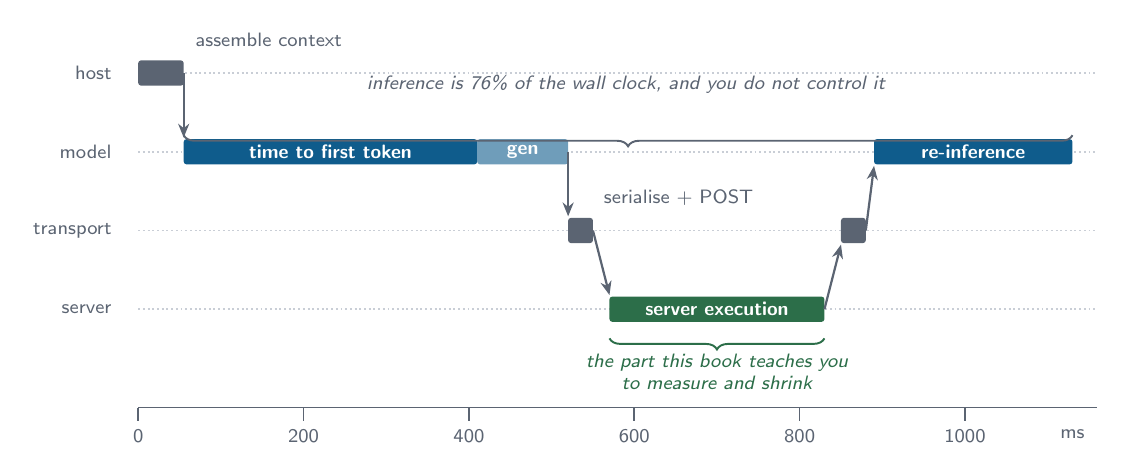
\begin{tikzpicture}[x=1.05cm, y=1cm]

  % ---- axis -------------------------------------------------------------
  \draw[tick] (0,-1.25) -- (11.6,-1.25);
  \foreach \x/\t in {0/0, 2/200, 4/400, 6/600, 8/800, 10/1000} {
    \draw[tick] (\x,-1.25) -- (\x,-1.42);
    \node[lbl, below=1pt] at (\x,-1.42) {\t};
  }
  \node[lbl, below=1pt] at (11.3,-1.42) {ms};

  % ---- bands ------------------------------------------------------------
  % y=3: host, y=2: model, y=1: transport, y=0: server
  \node[lbl, anchor=east] at (-0.25,3) {host};
  \node[lbl, anchor=east] at (-0.25,2) {model};
  \node[lbl, anchor=east] at (-0.25,1) {transport};
  \node[lbl, anchor=east] at (-0.25,0) {server};

  \foreach \y in {0,1,2,3} { \draw[lifeline] (0,\y) -- (11.6,\y); }

  % assemble context
  \barseg{0}{0.55}{3}{muted}{}
  \node[lbl, anchor=west] at (0.62,3.42) {assemble context};

  % inference to first token, then generation
  \barseg{0.55}{4.1}{2}{accent}{time to first token}
  \barseg{4.1}{5.2}{2}{accent!60}{gen}

  % serialize + transport out
  \barseg{5.2}{5.5}{1}{muted}{}
  \node[lbl, anchor=west] at (5.56,1.42) {serialise + POST};

  % server execution
  \barseg{5.7}{8.3}{0}{good}{server execution}

  % transport back
  \barseg{8.5}{8.8}{1}{muted}{}

  % re-inference
  \barseg{8.9}{11.3}{2}{accent}{re-inference}

  % ---- handoff arrows ---------------------------------------------------
  \draw[flowmuted] (0.55,3) -- (0.55,2.18);
  \draw[flowmuted] (5.2,2) -- (5.2,1.18);
  \draw[flowmuted] (5.5,1) -- (5.7,0.18);
  \draw[flowmuted] (8.3,0) -- (8.5,0.82);
  \draw[flowmuted] (8.8,1) -- (8.9,1.82);

  % ---- annotation -------------------------------------------------------
  \draw[decorate, decoration={brace, amplitude=4pt, raise=2pt}, muted, line width=0.7pt]
    (11.3,2.28) -- (0.55,2.28);
  \node[note, anchor=south] at (5.9,2.62)
    {inference is 76\% of the wall clock, and you do not control it};

  \draw[decorate, decoration={brace, mirror, amplitude=4pt, raise=2pt}, good, line width=0.7pt]
    (5.7,-0.30) -- (8.3,-0.30);
  \node[note, anchor=north, text=good, align=center] at (7.0,-0.44)
    {the part this book teaches you\\to measure and shrink};

\end{tikzpicture}
\end{document}
